% ============================================================
% PadPim: A Data-Driven 12-Key Flick Keyboard for
%         One-Handed Thai Input on Mobile Devices
% ============================================================
%
% COMPILATION (requires XeLaTeX for Thai Unicode support):
%   xelatex main.tex
%   bibtex  main
%   xelatex main.tex
%   xelatex main.tex
%
% REQUIREMENTS:
%   - XeLaTeX (included in MiKTeX / TeX Live)
%   - Thai font: Leelawadee UI (default on Windows 10/11)
%     or Noto Sans Thai (free from Google Fonts)
%   - Packages: tikz, pgfplots, booktabs, algorithm2e
%
% If you do not have Leelawadee UI, change \thaifont below
% to any Thai font installed on your system (e.g., Tahoma,
% Cordia New, TH Sarabun New, Noto Sans Thai).
% ============================================================

\documentclass[10pt,twocolumn,a4paper]{article}

% ---------- page geometry ----------
\usepackage[
  a4paper,
  left=1.8cm, right=1.8cm,
  top=2.2cm,  bottom=2.2cm,
  columnsep=0.6cm
]{geometry}

% ---------- fonts (XeLaTeX) ----------
\usepackage{fontspec}
\setmainfont{Times New Roman}[
  BoldFont   = Times New Roman Bold,
  ItalicFont = Times New Roman Italic,
]
\setsansfont{Arial}
\setmonofont{Consolas}
\newfontfamily\thaifont{Leelawadee UI}[Script=Thai]
\newcommand{\thai}[1]{{\thaifont #1}}

% ---------- language ----------
\usepackage{polyglossia}
\setdefaultlanguage{english}

% ---------- math ----------
\usepackage{amsmath,amssymb}

% ---------- graphics & color ----------
\usepackage{graphicx}
\usepackage[dvipsnames,svgnames,x11names,table]{xcolor}
\usepackage{tikz}
\usetikzlibrary{
  shapes.geometric,arrows.meta,positioning,calc,
  fit,backgrounds,decorations.pathreplacing,patterns
}
\usepackage{pgfplots}
\pgfplotsset{compat=1.18}

% ---------- tables ----------
\usepackage{booktabs}
\usepackage{multirow}
\usepackage{array}
\newcolumntype{C}[1]{>{\centering\arraybackslash}p{#1}}

% ---------- algorithms ----------
\usepackage[ruled,linesnumbered,noend]{algorithm2e}

% ---------- captions ----------
\usepackage[font=small,labelfont=bf]{caption}
\usepackage{subcaption}

% ---------- lists ----------
\usepackage{enumitem}
\setlist{nosep,leftmargin=*}

% ---------- hyperlinks ----------
\usepackage[hidelinks]{hyperref}
\usepackage{url}

% ---------- misc ----------
\usepackage{balance}  % balance last page columns
\usepackage{microtype}

% ---------- custom colors ----------
\definecolor{cHigh}{HTML}{EF4444}
\definecolor{cMid}{HTML}{F97316}
\definecolor{cMidLow}{HTML}{EAB308}
\definecolor{cLow}{HTML}{22C55E}
\definecolor{cSLow}{HTML}{94A3B8}
\definecolor{cVowel}{HTML}{EC4899}
\definecolor{cConBlue}{HTML}{6366F1}
\definecolor{cConGreen}{HTML}{22C55E}
\definecolor{cConYellow}{HTML}{F59E0B}
\definecolor{cGray}{HTML}{64748B}

% ---------- section formatting ----------
\usepackage{titlesec}
\titleformat{\section}{\large\bfseries}{\thesection.}{0.5em}{}
\titleformat{\subsection}{\normalsize\bfseries}{\thesubsection}{0.5em}{}
\titlespacing*{\section}{0pt}{1.2ex plus 0.4ex minus 0.2ex}{0.6ex plus 0.2ex}
\titlespacing*{\subsection}{0pt}{0.8ex plus 0.3ex minus 0.1ex}{0.4ex plus 0.1ex}

% ---------- title formatting ----------
\makeatletter
\renewcommand{\maketitle}{%
  \twocolumn[%
    \begin{center}
      {\LARGE\bfseries \@title \par}
      \vskip 1em
      {\large \@author \par}
      \vskip 0.5em
      {\normalsize \@date \par}
      \vskip 1.5em
    \end{center}
  ]%
}
\makeatother

% ============================================================
\begin{document}

\title{From 69 Characters to 12 Keys: A Corpus-Driven\\
Flick Keyboard for One-Handed Thai Mobile Input}

\author{
  Chawabhon Netisingha\\
  \textit{Independent Researcher}\\
  \texttt{Jn03official@gmail.com}
}

\date{}
\maketitle

% ============================================================
% ABSTRACT
% ============================================================
\begin{abstract}
Thai script requires a repertoire of 69~characters---44~consonants, 21~vowel and diphthong forms, and 4~tone marks---yet mobile Thai input still relies on miniaturized QWERTY layouts originally designed for two-handed desktop typing.
We present \textbf{PadPim}, to our knowledge the first frequency-optimized 12-key flick keyboard for Thai, adapting the Japanese \emph{kana} flick-input paradigm to Thai script.
We describe a complete data-driven pipeline: character frequency analysis from a corpus of over one million lines of Thai conversation collected from 138~university students, a position-scoring model that combines grid ergonomics with flick-direction ease of use, and a greedy optimization algorithm that assigns 57~characters to 12~keys with 5~flick directions each.
The 57~main-page characters and 3~space-key tone marks together cover approximately \textbf{97.5\%} of Thai character occurrences; only 9~characters ($\sim$0.1\% of text) require a shift layer.
We present two layout variants---\emph{PadPim-Opti} (pure frequency optimization) and \emph{PadPim-Key} (vowel-grouped for learnability)---and compare them against the Kedmanee and Pattachote QWERTY baselines on theoretical efficiency metrics including keys-per-character, touch-target area, and shift frequency.
PadPim is implemented as an open-source Android input-method editor and is available for public beta testing.
\end{abstract}

\medskip
\noindent\textbf{Keywords:} Thai keyboard, flick input, mobile text entry, keyboard layout optimization, one-handed input, character frequency analysis

% ============================================================
\section{Introduction}
\label{sec:intro}
% ============================================================

Mobile text entry in Thai poses a unique challenge.
The Thai script uses 69~distinct characters: 44~consonants, 21~vowel and diphthong forms (some written before, above, below, or after the base consonant), and 4~tone marks that alter pronunciation~\cite{aroonmanakun2002}.
The standard \emph{Kedmanee} keyboard layout, designed in 1968 for mechanical typewriters, maps these characters onto 47~keys spread across two shift layers.
On a modern smartphone, those 47~keys shrink to touch targets as small as 6\,mm wide---well below the 9.2\,mm recommended minimum for reliable thumb input~\cite{bergstrom2014}.
Users must frequently toggle shift to access common vowels and tone marks, adding cognitive load and motor overhead.

In Japan, a radically different solution has become the dominant mobile input method: the \textbf{12-key flick keyboard}.
Instead of replicating the full desktop layout, Japanese mobile input groups the 46~hiragana characters into 10~consonant-family keys arranged in a compact grid.
Each key produces five characters via five gestures: a center \emph{tap} and four directional \emph{flicks} (up, down, left, right).
This design yields large touch targets, single-hand operability, and a one-to-one mapping between gesture and character---no multi-tap ambiguity.

Despite the success of flick input for Japanese, \textbf{to our knowledge no prior work has adapted this paradigm to Thai script}.
Thai, with 69~characters, is a natural candidate: the character count is comparable to Japanese kana, and the characters can be partitioned into groups that fit a 12-key $\times$ 5-direction grid (60~slots on the main page).

In this paper we present \textbf{PadPim}\footnote{From Thai \thai{แพด} (\emph{pad}, touchpad) + \thai{พิมพ์} (\emph{pim}, to type).}, a data-driven 12-key flick keyboard for Thai.
Our contributions are:

\begin{enumerate}
  \item \textbf{Thai flick keyboard}: to our knowledge, the first application of the 12-key flick paradigm to Thai script, achieving 97.5\% one-action character coverage.
  \item \textbf{Data-driven layout pipeline}: we collect character frequencies from over one million lines of modern Thai conversation, derive a position-scoring model, and apply a greedy optimization algorithm to assign characters to key positions.
  \item \textbf{Two layout variants}: \emph{PadPim-Opti} maximizes typing efficiency via pure frequency optimization; \emph{PadPim-Key} groups vowels onto dedicated keys for faster learning.
  \item \textbf{Open-source implementation}: PadPim is released as an Android input-method editor, currently in public beta.
\end{enumerate}

% --- Figure 1: Japanese flick paradigm ---
\begin{figure}[t]
\centering
\begin{tikzpicture}[
  key/.style={
    draw, rounded corners=2pt, minimum width=1.0cm,
    minimum height=0.8cm, font=\scriptsize, align=center,
    fill=blue!6
  },
  flabel/.style={font=\scriptsize\sffamily,text=gray!70!black},
]
% 3x4 grid for Japanese kana (compact)
\foreach \r/\row in {0/{a,ka,sa},1/{ta,na,ha},2/{ma,ya,ra},3/{wa,--,nn}}{
  \foreach \c [count=\ci from 0] in \row {
    \node[key] (k\r\ci) at (\ci*1.2, -\r*1.0) {\c};
  }
}
% Callout for flick directions
\node[key,fill=orange!10,minimum width=1.6cm,minimum height=1.6cm]
  (demo) at (4.6,-0.8) {\large a};
\node[flabel,above=0.25cm of demo] {i};
\node[flabel,below=0.25cm of demo] {o};
\node[flabel,left=0.25cm of demo]  {u};
\node[flabel,right=0.25cm of demo] {e};
\draw[-{Stealth},gray,thick] (demo.north) -- ++(0,0.25);
\draw[-{Stealth},gray,thick] (demo.south) -- ++(0,-0.25);
\draw[-{Stealth},gray,thick] (demo.west)  -- ++(-0.25,0);
\draw[-{Stealth},gray,thick] (demo.east)  -- ++(0.25,0);
\node[above=0.6cm of demo,font=\scriptsize\sffamily\bfseries] {Flick directions};
\end{tikzpicture}
\caption{The Japanese 12-key flick keyboard groups 46 hiragana into consonant-family keys. Each key maps 5~characters to a tap and four flick directions (right callout). PadPim adapts this paradigm for Thai script.}
\label{fig:japanese_flick}
\end{figure}

% ============================================================
\section{Background and Related Work}
\label{sec:background}
% ============================================================

\subsection{Thai Script and Existing Input Methods}
\label{sec:bg_thai}

Thai is an abugida written left-to-right without inter-word spaces~\cite{aroonmanakun2002}.
Its 44~consonants represent initial and final consonant sounds; 21~vowel forms combine as prefixed, suffixed, superscript, or subscript glyphs around a base consonant; and 4~tone marks (\thai{่\, ้\, ๊\, ๋}) are placed above the consonant to indicate lexical tone~\cite{aroonmanakun2002}.

The \textbf{Kedmanee} layout, the \emph{de facto} standard, was designed by Sawasdee Sukkasame in 1968 for the IBM Selectric typewriter.
It distributes 69~characters across 47~physical keys with a two-layer shift mapping.
While adequate for full-size keyboards, the layout was never optimized for frequency or ergonomics.

The \textbf{Pattachote} layout, proposed by Sarakit Pattachote in 1986, rearranges the character assignments based on frequency analysis and places high-frequency characters on the home row.
Despite demonstrated efficiency gains, Pattachote never achieved mainstream adoption due to the installed base of Kedmanee.

On mobile, Thai users predominantly type on miniaturized Kedmanee QWERTY keyboards provided by Gboard, Samsung Keyboard, and SwiftKey.
These layouts inherit all the desktop-era limitations---small keys, frequent shifting, two-handed design---compounded by the constraints of a 6-inch touchscreen.

\subsection{Flick Input on 12-Key Keypads}
\label{sec:bg_flick}

The 12-key phone keypad has been used for text input since the advent of SMS.
Early approaches used \emph{multi-tap}---pressing a key multiple times to cycle through associated characters---and \emph{T9} predictive disambiguation~\cite{grover1998,silfverberg2000}.
Both suffer from ambiguity or multi-press overhead.

The \textbf{flick keyboard} eliminates these issues by mapping each character to a unique gesture: a center tap or a directional flick (up, down, left, right) on one of 10--12 keys.
Introduced on the Apple iPhone in 2008 for Japanese \emph{kana} input and popularized by Google Japanese Input, flick keyboards have become the dominant mobile input method in Japan.

Flick input offers several advantages over QWERTY on mobile:
(1)~\emph{large touch targets}, since 12~keys occupy the same screen area as 30+ QWERTY keys;
(2)~\emph{one-handed operability}, since the compact grid fits within the thumb's functional reach~\cite{karlson2006,bergstrom2014};
(3)~\emph{unambiguous input}, since every character maps to exactly one gesture.

To our knowledge, the paradigm has not been applied to Thai.

\subsection{Keyboard Layout Optimization}
\label{sec:bg_optim}

Layout optimization for touchscreen keyboards is well-studied.
Fitts' law~\cite{fitts1954} predicts that movement time to a target depends on its distance and width; smaller, farther keys are slower to reach.
Zhai et~al.~\cite{zhai2002} optimized QWERTY-like layouts by minimizing Fitts'-law movement costs between character pairs.
Bi et~al.~\cite{bi2012} extended this to multilingual keyboards.
Oulasvirta et~al.~\cite{oulasvirta2013} used combinatorial optimization to design the KALQ split-thumb keyboard.
Dunlop and Levine~\cite{dunlop2012} applied multi-objective Pareto optimization balancing speed, familiarity, and error correction.

These prior works focus on QWERTY-like layouts with one character per key.
In contrast, our work optimizes a \emph{flick keyboard} where each key maps five characters via directional gestures, introducing a second dimension---flick-direction difficulty---into the scoring model.

% ============================================================
\section{Data Collection and Character Frequency Analysis}
\label{sec:data}
% ============================================================

\subsection{Corpus Collection}
\label{sec:data_corpus}

To design a keyboard layout optimized for modern Thai communication, we collected character frequency data from real conversational text rather than relying solely on published corpora from formal sources.

We recruited \textbf{138~Thai university students} (age range 18--25) who voluntarily contributed anonymized character frequency counts extracted from their personal messaging conversations.
Source platforms included LINE, Facebook Messenger, WhatsApp, Discord, and Twitter (now X) direct messages.
The resulting corpus comprises over \textbf{1,000,000~lines} of Thai conversational text.

\textbf{Ethics and privacy.}
To protect participant privacy, we employed a two-stage anonymization protocol:
(1)~participants ran a local character-counting script on their own devices, producing only aggregated per-character frequency counts;
(2)~only these anonymous numerical counts were transmitted to the researchers---no raw message text was ever collected or stored.
Informed consent was obtained from all participants.

\subsection{Processing Pipeline}
\label{sec:data_pipeline}

\begin{figure}[t]
\centering
\begin{tikzpicture}[
  box/.style={
    draw, rounded corners=3pt, fill=blue!5,
    minimum width=2.2cm, minimum height=0.7cm,
    font=\scriptsize\sffamily, align=center
  },
  arr/.style={-{Stealth},thick,gray!70},
  filt/.style={
    draw, rounded corners=2pt, fill=red!8,
    minimum width=1.8cm, minimum height=0.55cm,
    font=\scriptsize\sffamily, align=center
  },
]
\node[box] (raw) {Raw chat\\messages};
\node[filt,right=0.4cm of raw] (f1) {Remove\\URLs};
\node[filt,right=0.4cm of f1] (f2) {Remove\\emoji};
\node[box,below=0.5cm of f2]  (f3) {Filter\\English};
\node[box,left=0.4cm of f3]   (ext) {Thai char\\extraction};
\node[box,left=0.4cm of ext]  (cnt) {Frequency\\counting};
\node[box,below=0.5cm of cnt] (out) {Normalized\\distribution};

\draw[arr] (raw) -- (f1);
\draw[arr] (f1)  -- (f2);
\draw[arr] (f2)  -- (f3);
\draw[arr] (f3)  -- (ext);
\draw[arr] (ext) -- (cnt);
\draw[arr] (cnt) -- (out);
\end{tikzpicture}
\caption{Data processing pipeline. Raw conversation text is filtered to remove non-Thai content, then Thai characters are extracted and counted to produce a normalized frequency distribution.}
\label{fig:pipeline}
\end{figure}

The processing pipeline (Figure~\ref{fig:pipeline}) operates as follows:

\begin{enumerate}
  \item \textbf{URL and link removal}: Regular expressions strip HTTP(S) links and shortened URLs.
  \item \textbf{Emoji and sticker removal}: Unicode emoji ranges (U+1F600--U+1F9FF, etc.) are filtered out.
  \item \textbf{English and number filtering}: Non-Thai script (Latin, digits, CJK) is removed based on Unicode block detection (Thai block: U+0E00--U+0E7F).
  \item \textbf{Thai character extraction}: Remaining text is segmented into individual Thai characters, distinguishing base consonants, vowel forms, tone marks, and diacritics~\cite{theeramunkong2001}.
  \item \textbf{Frequency counting}: Per-character absolute counts are computed across all participants, then normalized to percentages.
\end{enumerate}

A combination of automated scripts and manual verification was used to ensure data quality, particularly for edge cases involving mixed-script messages and informal transliterations.

\subsection{Frequency Results}
\label{sec:data_results}

Table~\ref{tab:freq} presents the 30~most frequent Thai characters in our corpus.
The most frequent character is \thai{า} (\emph{sara aa}) at 7.12\%, followed by \thai{ร} (\emph{ro rua}) at 6.49\% and \thai{น} (\emph{no nu}) at 6.08\%.

\begin{table}[t]
\centering
\caption{Top 30 Thai characters by frequency in our corpus of 1M+ lines of conversational text from 138 participants.}
\label{tab:freq}
\small
\begin{tabular}{@{}rlllr@{}}
\toprule
\textbf{Rank} & \textbf{Char} & \textbf{Name} & \textbf{Type} & \textbf{Freq\,\%} \\
\midrule
 1 & \thai{า}  & Sara aa       & Vowel & 7.12 \\
 2 & \thai{ร}  & Ro rua        & Cons. & 6.49 \\
 3 & \thai{น}  & No nu         & Cons. & 6.08 \\
 4 & \thai{ก}  & Ko kai        & Cons. & 4.42 \\
 5 & \thai{อ}  & O ang         & Cons. & 3.96 \\
 6 & \thai{เ}  & Sara e        & Vowel & 3.81 \\
 7 & \thai{ง}  & Ngo ngu       & Cons. & 3.80 \\
 8 & \thai{◌ั} & Sara an       & Vowel & 3.28 \\
 9 & \thai{ม}  & Mo ma         & Cons. & 3.24 \\
10 & \thai{ย}  & Yo yak        & Cons. & 3.22 \\
11 & \thai{ว}  & Wo waen       & Cons. & 2.65 \\
12 & \thai{◌ี} & Sara ii       & Vowel & 2.64 \\
13 & \thai{ท}  & Tho thahan    & Cons. & 2.50 \\
14 & \thai{ด}  & Do chada      & Cons. & 2.32 \\
15 & \thai{ล}  & Lo ling       & Cons. & 2.29 \\
16 & \thai{◌ิ} & Sara i        & Vowel & 2.06 \\
17 & \thai{ต}  & To tao        & Cons. & 1.99 \\
18 & \thai{ะ}  & Sara a        & Vowel & 1.81 \\
19 & \thai{ป}  & Po pla        & Cons. & 1.69 \\
20 & \thai{จ}  & Jo jan        & Cons. & 1.64 \\
21 & \thai{ค}  & Kho khwai     & Cons. & 1.62 \\
22 & \thai{ห}  & Ho hip        & Cons. & 1.55 \\
23 & \thai{ส}  & So suea       & Cons. & 1.51 \\
24 & \thai{แ}  & Sara ae       & Vowel & 1.29 \\
25 & \thai{◌์} & Thanthakhat   & Diacr.& 1.20 \\
26 & \thai{ไ}  & Sara ai mai   & Vowel & 1.20 \\
27 & \thai{พ}  & Pho phan      & Cons. & 1.14 \\
28 & \thai{ข}  & Kho khai      & Cons. & 1.14 \\
29 & \thai{ใ}  & Sara ai muan  & Vowel & 1.08 \\
30 & \thai{ช}  & Cho chang     & Cons. & 1.07 \\
\bottomrule
\end{tabular}
\end{table}

% --- Figure 3: Frequency bar chart ---
\begin{figure*}[t]
\centering
\begin{tikzpicture}
\begin{axis}[
  ybar,
  bar width=6pt,
  width=\textwidth,
  height=5.5cm,
  ylabel={Frequency (\%)},
  ylabel style={font=\small},
  ymin=0, ymax=8,
  xtick=data,
  symbolic x coords={
    {\thai{า}},{\thai{ร}},{\thai{น}},{\thai{ก}},{\thai{อ}},
    {\thai{เ}},{\thai{ง}},{\thai{ั}},{\thai{ม}},{\thai{ย}},
    {\thai{ว}},{\thai{ี}},{\thai{ท}},{\thai{ด}},{\thai{ล}},
    {\thai{ิ}},{\thai{ต}},{\thai{ะ}},{\thai{ป}},{\thai{จ}},
    {\thai{ค}},{\thai{ห}},{\thai{ส}},{\thai{แ}},{\thai{์}},
    {\thai{ไ}},{\thai{พ}},{\thai{ข}},{\thai{ใ}},{\thai{ช}}
  },
  xticklabel style={font=\thaifont\small},
  x tick label style={rotate=0},
  xlabel={Thai character},
  xlabel style={font=\small},
  ytick={0,1,2,3,4,5,6,7,8},
  yticklabel style={font=\scriptsize},
  grid=major,
  grid style={gray!20},
  every axis plot/.append style={fill=cConBlue!70,draw=cConBlue},
  nodes near coords,
  nodes near coords style={font=\tiny,rotate=90,anchor=west,xshift=0pt,yshift=1pt},
  every node near coord/.append style={/pgf/number format/.cd,fixed,precision=1},
  enlarge x limits=0.02,
]
\addplot coordinates {
  ({\thai{า}},7.12) ({\thai{ร}},6.49) ({\thai{น}},6.08) ({\thai{ก}},4.42)
  ({\thai{อ}},3.96) ({\thai{เ}},3.81) ({\thai{ง}},3.80) ({\thai{ั}},3.28)
  ({\thai{ม}},3.24) ({\thai{ย}},3.22) ({\thai{ว}},2.65) ({\thai{ี}},2.64)
  ({\thai{ท}},2.50) ({\thai{ด}},2.32) ({\thai{ล}},2.29) ({\thai{ิ}},2.06)
  ({\thai{ต}},1.99) ({\thai{ะ}},1.81) ({\thai{ป}},1.69) ({\thai{จ}},1.64)
  ({\thai{ค}},1.62) ({\thai{ห}},1.55) ({\thai{ส}},1.51) ({\thai{แ}},1.29)
  ({\thai{์}},1.20) ({\thai{ไ}},1.20) ({\thai{พ}},1.14) ({\thai{ข}},1.14)
  ({\thai{ใ}},1.08) ({\thai{ช}},1.07)
};
\end{axis}
\end{tikzpicture}
\caption{Character frequency distribution for the top 30 Thai characters in our conversational corpus. The distribution exhibits a Zipf-like curve: the top 10 characters account for 45.4\% of all Thai character usage, while the top 30 cover 82.8\%.}
\label{fig:freq_chart}
\end{figure*}

\textbf{Validation against published data.}
We compared our conversational frequency distribution against the formal-text frequencies published by Aroonmanakun~\cite{aroonmanakun2006}, who analyzed a corpus of approximately 354~million Thai characters from mixed published sources.
The Spearman rank-order correlation between the two distributions is $\rho = 0.97$ ($p < 0.001$), with the top~10 characters appearing in nearly identical order.
This strong concordance suggests that Thai character frequencies are relatively stable across registers (formal vs.\ informal) and time periods (2006 vs.\ 2024), validating the use of modern conversational data for layout design.

The frequency distribution exhibits a Zipf-like shape (Figure~\ref{fig:freq_chart}): the top~10 characters account for 45.4\% of all usage, and the top~30 cover 82.8\%.
This heavy concentration at the top of the distribution is precisely what makes a 12-key flick layout viable---the majority of typing involves a small subset of characters that can be placed on the most accessible key positions.

% ============================================================
\section{Layout Design Methodology}
\label{sec:design}
% ============================================================

Our layout design proceeds in four stages: (1)~define the grid structure, (2)~score each position by ergonomic accessibility, (3)~assign characters to positions via a greedy algorithm, and (4)~handle special cases (tone marks, rare characters).

\subsection{Grid Structure}
\label{sec:design_grid}

PadPim arranges \textbf{12~character keys} in a $3 \times 4$ grid (3~columns, 4~rows), flanked by utility keys on each side (Figure~\ref{fig:heatmap}).
The left column holds input-mode controls (microphone, cursor-left, language switch, shift/emoji); the right column holds action keys (backspace, cursor-right, space, enter).
This yields a full $5 \times 4$ grid on the keyboard surface, with the central $3 \times 4$ block dedicated to character input.

Each character key supports \textbf{5~input gestures}: a center \emph{tap} and four directional \emph{flicks} (up, down, left, right).
The bottom row (row~3) omits the down-flick because keys at the screen edge have no room for downward gesture travel, yielding:
$$
N_{\text{slots}} = 3 \times 3 \times 5 + 3 \times 1 \times 4 = 45 + 12 = 57
$$
Thus, 57~characters can be placed on the main page without any shift layer.

\subsection{Position Scoring Model}
\label{sec:design_scoring}

We assign each of the 57~character positions a \textbf{combined score} that reflects how easy it is for the user's thumb to reach.
The score has two components: a \emph{grid score} and a \emph{flick multiplier}.

\textbf{Grid score.}
Based on ergonomic thumb-reach studies~\cite{bergstrom2014,karlson2006} and our own week-long empirical testing with a prototype, we assigned grid scores to each key position (Figure~\ref{fig:heatmap}).
The center key of the middle row (row~1, col~2) receives the highest score of 100---it lies at the natural thumb resting position.
Adjacent mid-row keys score 80; top-row and lower-row keys score 40--60; the bottom row scores 20.

\textbf{Flick multiplier.}
Not all flick directions are equally easy.
Through empirical testing with a prototype over one week and informed by Japanese flick-keyboard ergonomics research, we determined the following multipliers:

\begin{itemize}
  \item \textbf{Tap} (center): $1.0$ --- the default, easiest action
  \item \textbf{Up}: $0.8$ --- natural upward thumb extension
  \item \textbf{Left / Right}: $0.6$ --- lateral thumb movement
  \item \textbf{Down}: $0.4$ --- least natural; opposes gravity for the thumb
\end{itemize}

\textbf{Combined score.}
For a key at grid position $(r, c)$ with flick direction $d$:
\begin{equation}
  S(r, c, d) = G(r, c) \times M(d)
  \label{eq:score}
\end{equation}
where $G(r,c)$ is the grid score and $M(d)$ is the flick multiplier.
For example, a tap on the center key scores $100 \times 1.0 = 100$, while a left-flick on a bottom-row key scores $20 \times 0.6 = 12$.

% --- Figure 4: Position scoring heatmap ---
\begin{figure}[t]
\centering
\begin{tikzpicture}[
  cell/.style={
    minimum width=1.3cm, minimum height=0.95cm,
    font=\scriptsize\sffamily\bfseries, align=center,
    rounded corners=2pt
  },
  util/.style={cell, fill=gray!15, text=gray!60, font=\tiny\sffamily},
  h100/.style={cell, fill=cHigh!60, text=white},
  h80/.style={cell, fill=cMid!50},
  h60/.style={cell, fill=cMidLow!45},
  h40/.style={cell, fill=cLow!35},
  h20/.style={cell, fill=cSLow!30},
]
% Row 0
\node[util] at (0,0) {mic};
\node[h40]  at (1.45,0) {40\\low};
\node[h60]  at (2.90,0) {60\\mid};
\node[h40]  at (4.35,0) {40\\low};
\node[util] at (5.80,0) {del};
% Row 1
\node[util] at (0,-1.1) {$<$};
\node[h80]  at (1.45,-1.1) {80\\mid};
\node[h100] at (2.90,-1.1) {100\\HIGH};
\node[h80]  at (4.35,-1.1) {80\\mid};
\node[util] at (5.80,-1.1) {$>$};
% Row 2
\node[util] at (0,-2.2) {lang};
\node[h40]  at (1.45,-2.2) {40\\low};
\node[h60]  at (2.90,-2.2) {60\\mid};
\node[h40]  at (4.35,-2.2) {40\\low};
\node[util] at (5.80,-2.2) {spc};
% Row 3
\node[util] at (0,-3.3) {shift};
\node[h20]  at (1.45,-3.3) {20\\s.low};
\node[h20]  at (2.90,-3.3) {20\\s.low};
\node[h20]  at (4.35,-3.3) {20\\s.low};
\node[util] at (5.80,-3.3) {ent};
\end{tikzpicture}
\caption{Position scoring heatmap for the $5 \times 4$ keyboard grid. The central $3 \times 4$ block contains character keys scored by ergonomic thumb reach: \textcolor{cHigh}{\textbf{100}} (center, optimal), \textcolor{cMid}{\textbf{80}} (mid-row), \textcolor{cMidLow}{\textbf{60}}/\textcolor{cLow}{\textbf{40}} (top/lower rows), \textcolor{cSLow}{\textbf{20}} (bottom row). Utility keys (gray) flank each side.}
\label{fig:heatmap}
\end{figure}

% --- Figure 5: Flick direction multipliers ---
\begin{figure}[t]
\centering
\begin{tikzpicture}[
  dir/.style={
    circle, draw=gray!50, fill=white,
    minimum size=0.8cm, font=\small\sffamily\bfseries,
    inner sep=0
  },
]
% Center
\node[dir,fill=cHigh!20,draw=cHigh!60] (C) at (0,0) {1.0};
% Directions
\node[dir,fill=cMid!20,draw=cMid!60]    (U) at (0, 1.3) {0.8};
\node[dir,fill=cMidLow!20,draw=cMidLow!60] (L) at (-1.3,0) {0.6};
\node[dir,fill=cMidLow!20,draw=cMidLow!60] (R) at ( 1.3,0) {0.6};
\node[dir,fill=cLow!20,draw=cLow!60]    (D) at (0,-1.3) {0.4};
% Arrows
\draw[-{Stealth},thick,cHigh!70] (C.north) -- (U.south);
\draw[-{Stealth},thick,cHigh!70] (C.south) -- (D.north);
\draw[-{Stealth},thick,cHigh!70] (C.west)  -- (L.east);
\draw[-{Stealth},thick,cHigh!70] (C.east)  -- (R.west);
% Labels
\node[above=0.15cm of U,font=\scriptsize\sffamily] {Up};
\node[below=0.15cm of D,font=\scriptsize\sffamily] {Down};
\node[left=0.15cm of L,font=\scriptsize\sffamily]  {Left};
\node[right=0.15cm of R,font=\scriptsize\sffamily] {Right};
\node[below right=0.1cm of C,font=\scriptsize\sffamily] {Tap};
\end{tikzpicture}
\caption{Flick direction multipliers. The tap (center) is easiest ($1.0$); upward flick ($0.8$) is natural for the thumb; lateral flicks ($0.6$) require more effort; downward flick ($0.4$) is hardest.}
\label{fig:flick_mult}
\end{figure}

\subsection{Greedy Assignment Algorithm}
\label{sec:design_greedy}

Given the 57~scored positions and 57~characters sorted by frequency, we apply a \textbf{greedy assignment} (Algorithm~\ref{alg:greedy}): the highest-frequency character is assigned to the highest-scoring position, the second-highest to the second-highest position, and so on.

This greedy approach is provably optimal under the assumption that each character is typed independently (i.e., no bigram transition costs).
By the \emph{rearrangement inequality}~\cite{hardy1952}, pairing the two sequences in matching sorted order maximizes $\sum_i f_i \cdot s_i$, the frequency-weighted total score.
Concretely: if $f_1 \geq f_2 \geq \cdots$ and $s_1 \geq s_2 \geq \cdots$, then for any permutation $\sigma$, $\sum_i f_i \, s_i \geq \sum_i f_i \, s_{\sigma(i)}$, so the identity permutation---the greedy zip---is optimal under the independence assumption.

\begin{algorithm}[t]
\caption{Greedy Character Assignment}
\label{alg:greedy}
\SetAlgoLined
\KwIn{Characters $C = \{c_1, \ldots, c_{57}\}$ with frequencies $f_i$\\
\quad\quad\; Positions $P = \{p_1, \ldots, p_{57}\}$ with scores $s_j$}
\KwOut{Assignment $A: C \rightarrow P$}
Sort $C$ by descending frequency: $f_1 \geq f_2 \geq \cdots$\;
Sort $P$ by descending score: $s_1 \geq s_2 \geq \cdots$\;
\For{$i = 1$ \KwTo $57$}{
  $A(c_i) \leftarrow p_i$\;
}
\Return{$A$}\;
\end{algorithm}

\subsection{Special Handling}
\label{sec:design_special}

\textbf{Tone marks on the space key.}
The three most common tone marks---\thai{่}~(\emph{mai ek}, 2.50\%), \thai{้}~(\emph{mai tho}, 1.80\%), and \thai{๊}~(\emph{mai tri}, 0.15\%)---are placed on the \emph{space key} as left, up, and right flicks, respectively.
This design is motivated by the observation that tone marks almost always follow a consonant; after typing the preceding consonant with the left hand area, the thumb naturally returns toward the space bar region.
Placing tones on the space key frees three valuable main-grid positions for consonants and vowels.

\textbf{Shift page for rare characters.}
The 9~rarest Thai characters---\thai{ฆ}~(0.03\%), \thai{๋}~(0.02\%), \thai{ฺ}~(0.01\%), \thai{ฌ}~(0.01\%), \thai{ฬ}~(0.01\%), \thai{ฮ}~($<$0.01\%), \thai{ฃ}, \thai{ฅ}, \thai{ฦ}~($\approx$0\%)---are relegated to a shift layer accessible via a dedicated shift key.
These characters collectively account for only $\sim$0.1\% of Thai text, meaning the shift key is almost never needed in practice.

\textbf{Coverage summary.}
These three character sets are mutually exclusive---no character appears on more than one layer:
\begin{itemize}
  \item Main page: 57~characters ($\sim$93\% of Thai character occurrences)
  \item Space-key tones: 3~tone marks ($\sim$4.5\%)
  \item Shift page: 9~rare characters ($\sim$0.1\%)
\end{itemize}
Together, the main page and space-key tones account for approximately 97.5\% of Thai character occurrences.
All 69~Thai characters are accessible across the three layers.

% ============================================================
\section{Layout Variants}
\label{sec:variants}
% ============================================================

We present two layout variants that trade off between raw typing efficiency and learnability.

\subsection{PadPim-Opti: Pure Frequency Optimization}
\label{sec:opti}

PadPim-Opti is the direct output of the greedy algorithm: every character is placed strictly according to its frequency-to-score rank.
Figure~\ref{fig:layout_opti} shows the complete layout.

The highest-frequency character, \thai{า} (7.12\%), occupies the center tap of the highest-scoring key (row~1, col~2, score~100).
The second-highest, \thai{ร} (6.49\%), takes the up-flick of the same key (score~80).
Characters are distributed across all 12~keys purely by the greedy assignment.

\textbf{Advantage}: PadPim-Opti achieves the theoretically maximum frequency-weighted position score---it is the fastest layout for experienced users.

\textbf{Disadvantage}: vowels and consonants are intermixed across keys with no categorical grouping, making the layout harder to learn initially.

% --- Figure 6: PadPim-Opti layout ---
\begin{figure}[t]
\centering
\renewcommand{\arraystretch}{1.15}
\footnotesize
\begin{tabular}{|C{2.0cm}|C{2.0cm}|C{2.0cm}|}
\hline
\multicolumn{3}{|c|}{\textbf{Row 0} (low priority)} \\
\hline
\thai{ข} & \thai{ล} & \thai{ใ} \\
\thai{ธ}\;\textbf{\thai{ะ}}\;\thai{ผ} &
\thai{ห}\;\textbf{\thai{ม}}\;\thai{ส} &
\thai{ู}\;\textbf{\thai{ป}}\;\thai{็} \\
\thai{ึ} & \thai{ุ} & \thai{ฟ} \\
\hline
\multicolumn{3}{|c|}{\textbf{Row 1} (highest priority)} \\
\hline
\thai{อ} & \thai{ร} & \thai{เ} \\
\thai{ว}\;\textbf{\thai{น}}\;\thai{ี} &
\thai{ง}\;\textbf{\thai{า}}\;\thai{ั} &
\thai{ท}\;\textbf{\thai{ก}}\;\thai{ด} \\
\thai{ไ} & \thai{ต} & \thai{พ} \\
\hline
\multicolumn{3}{|c|}{\textbf{Row 2} (low priority)} \\
\hline
\thai{ช} & \thai{ิ} & \thai{ื} \\
\thai{ำ}\;\textbf{\thai{จ}}\;\thai{ณ} &
\thai{แ}\;\textbf{\thai{ย}}\;\thai{์} &
\thai{ศ}\;\textbf{\thai{ค}}\;\thai{ถ} \\
\thai{ญ} & \thai{บ} & \thai{ภ} \\
\hline
\multicolumn{3}{|c|}{\textbf{Row 3} (super-low, no down-flick)} \\
\hline
\thai{ๆ} & \thai{ฉ} & \thai{ฒ} \\
\thai{ฯ}\;\textbf{\thai{โ}}\;\thai{ฎ} &
\thai{ฏ}\;\textbf{\thai{ซ}}\;\thai{ฐ} &
\thai{ฤ}\;\textbf{\thai{ษ}}\;\thai{ฑ} \\
\hline
\end{tabular}
\caption{PadPim-Opti layout. Each cell shows: \emph{top}=up-flick, \emph{left} \textbf{center} \emph{right}=left-flick / tap / right-flick, \emph{bottom}=down-flick. Bold center character is the tap (highest priority per key). Characters are assigned purely by frequency-score matching.}
\label{fig:layout_opti}
\end{figure}

\subsection{PadPim-Key: Vowel-Grouped Variant}
\label{sec:key}

PadPim-Key addresses learnability by consolidating all vowels onto \textbf{two dedicated keys} (\thai{สระ~๑} and \thai{สระ~๒}, meaning ``Vowel~1'' and ``Vowel~2''), located at the center of the grid.
The remaining 10~keys hold consonants, assigned by greedy optimization within the consonant subset.

\begin{itemize}
  \item \textbf{Vowel Key 1} (row~1, col~2): \thai{า}, \thai{ั}, \thai{เ}, \thai{ี}, \thai{ะ}---the five most frequent vowels.
  \item \textbf{Vowel Key 2} (row~2, col~2): \thai{ิ}, \thai{ุ}, \thai{แ}, \thai{ู}, \thai{ำ}---the next five vowels.
\end{itemize}

\textbf{Advantage}: Users learn that ``vowels are always on these two pink keys,'' dramatically reducing visual search time for beginners.

\textbf{Disadvantage}: Grouping constrains the optimizer.  Some vowels are forced onto lower-scoring positions than they would occupy in the unconstrained (Opti) layout.

% --- Figure 7: PadPim-Key layout ---
\begin{figure}[t]
\centering
\renewcommand{\arraystretch}{1.15}
\footnotesize
\begin{tabular}{|C{2.0cm}|C{2.0cm}|C{2.0cm}|}
\hline
\multicolumn{3}{|c|}{\textbf{Row 0} (low priority)} \\
\hline
\thai{์} & \thai{ด} & \thai{พ} \\
\thai{ื}\;\textbf{\thai{ล}}\;\thai{บ} &
\thai{ค}\;\textbf{\thai{ง}}\;\thai{ห} &
\thai{ธ}\;\textbf{\thai{ต}}\;\thai{ผ} \\
\thai{ึ} & \thai{ช} & \thai{ฟ} \\
\hline
\multicolumn{3}{|c|}{\textbf{Row 1} (highest priority)} \\
\hline
\thai{ก} & \thai{เ} & \thai{อ} \\
\thai{ม}\;\textbf{\thai{ร}}\;\thai{ย} &
\cellcolor{cVowel!15}\thai{ั}\;\textbf{\thai{า}}\;\thai{ี}\;\textsuperscript{\sffamily\bfseries V\textsubscript{1}} &
\thai{ว}\;\textbf{\thai{น}}\;\thai{ท} \\
\thai{ส} & \cellcolor{cVowel!15}\thai{ะ} & \thai{ไ} \\
\hline
\multicolumn{3}{|c|}{\textbf{Row 2} (low priority)} \\
\hline
\thai{ข} & \thai{แ} & \thai{ใ} \\
\thai{็}\;\textbf{\thai{ป}}\;\thai{ณ} &
\cellcolor{cVowel!15}\thai{ุ}\;\textbf{\thai{ิ}}\;\thai{ู}\;\textsuperscript{\sffamily\bfseries V\textsubscript{2}} &
\thai{ศ}\;\textbf{\thai{จ}}\;\thai{ถ} \\
\thai{ญ} & \cellcolor{cVowel!15}\thai{ำ} & \thai{ภ} \\
\hline
\multicolumn{3}{|c|}{\textbf{Row 3} (super-low, no down-flick)} \\
\hline
\thai{ๆ} & \thai{ฉ} & \thai{ฒ} \\
\thai{ฯ}\;\textbf{\thai{โ}}\;\thai{ฎ} &
\thai{ฏ}\;\textbf{\thai{ซ}}\;\thai{ฐ} &
\thai{ฤ}\;\textbf{\thai{ษ}}\;\thai{ฑ} \\
\hline
\end{tabular}
\caption{PadPim-Key layout. The two dedicated vowel keys are marked \textsuperscript{\sffamily\bfseries V\textsubscript{1}} and \textsuperscript{\sffamily\bfseries V\textsubscript{2}} (shaded in color prints). All vowels are concentrated on these keys for faster learning; consonants fill the remaining 10~keys by frequency optimization.}
\label{fig:layout_key}
\end{figure}

\subsection{Variant Comparison}
\label{sec:variant_compare}

Table~\ref{tab:variant_compare} compares the two variants on frequency-weighted metrics.
We compute the \emph{weighted average score} as $\bar{S} = \sum_{i} f_i \cdot S_i$, where $f_i$ is the frequency and $S_i$ the position score of character~$i$.

\begin{table}[t]
\centering
\caption{Comparison of PadPim-Opti and PadPim-Key layout variants. Higher weighted score indicates better average ergonomic placement.}
\label{tab:variant_compare}
\small
\begin{tabular}{@{}lcc@{}}
\toprule
\textbf{Metric} & \textbf{PadPim-Opti} & \textbf{PadPim-Key} \\
\midrule
One-action coverage    & 97.5\%  & 97.5\% \\
Characters on main page & 57    & 57 \\
Weighted avg.\ score  & 62.4    & 58.7 \\
Top-10 char avg.\ score & 76.8  & 73.2 \\
Vowel avg.\ score     & 55.1    & 50.8 \\
Consonant avg.\ score & 65.3    & 62.9 \\
Vowel keys            & Distributed & 2 dedicated \\
Learning model        & Memorize all & Learn 2 vowel keys \\
\bottomrule
\end{tabular}
\end{table}

PadPim-Opti achieves a 6.3\% higher weighted average score than PadPim-Key.
However, PadPim-Key's categorical vowel grouping substantially reduces the cognitive search space: instead of scanning all 12~keys for a vowel, users need only check two fixed locations.
We hypothesize that PadPim-Key will exhibit a faster learning curve, while PadPim-Opti will yield higher peak performance for experienced users.

% ============================================================
\section{Theoretical Evaluation}
\label{sec:eval}
% ============================================================

In the absence of a formal user study---planned as future work (\S\ref{sec:future})---we evaluate PadPim using theoretical efficiency metrics and compare against two QWERTY baselines.

\subsection{Baselines}
\label{sec:eval_baselines}

\begin{itemize}
  \item \textbf{Kedmanee}: Standard Thai QWERTY layout. 47~keys, 2~shift layers. Used by the vast majority of Thai typists.
  \item \textbf{Pattachote}: Frequency-optimized Thai QWERTY layout. 47~keys, 2~shift layers. Positions high-frequency characters on the home row.
\end{itemize}

Both baselines are designed for full-size keyboards and assume two-handed typing.
On mobile, they are rendered as miniaturized touchscreen QWERTY layouts.

\subsection{Comparison Metrics}
\label{sec:eval_metrics}

Table~\ref{tab:comparison} presents the comparison.

\begin{table}[t]
\centering
\caption{Theoretical comparison of PadPim against Kedmanee and Pattachote baselines on a 6-inch (68\,mm wide) mobile display. Baseline KPC and shift-frequency values were derived by mapping our corpus onto each layout's key-to-character assignment and counting one-action vs.\ shifted character occurrences.}
\label{tab:comparison}
\small
\begin{tabular}{@{}lcccc@{}}
\toprule
 & \rotatebox{60}{\textbf{PadPim-O}} & \rotatebox{60}{\textbf{PadPim-K}} & \rotatebox{60}{\textbf{Kedmanee}} & \rotatebox{60}{\textbf{Pattachote}} \\
\midrule
Total keys           & 12  & 12  & 47  & 47  \\
Shift layers         & 1   & 1   & 2   & 2   \\
Chars/key (max)      & 5   & 5   & 1   & 1   \\
One-hand capable     & Yes & Yes & No  & No  \\
\midrule
\multicolumn{5}{@{}l}{\textit{Coverage \& efficiency}} \\
\midrule
One-action coverage   & 97.5\% & 97.5\% & $\sim$55\% & $\sim$55\% \\
Avg.\ KPC            & 1.001  & 1.001  & 1.29  & 1.25 \\
Shift freq.\ /100 chars & 0.1 & 0.1 & $\sim$29 & $\sim$25 \\
\midrule
\multicolumn{5}{@{}l}{\textit{Touch target (6-inch screen)}} \\
\midrule
Key width (mm)       & 13.6 & 13.6 & 5.8 & 5.8 \\
Key area (mm$^2$)    & 184  & 184  & 44  & 44  \\
Area ratio           & 4.2$\times$ & 4.2$\times$ & 1$\times$ & 1$\times$ \\
\bottomrule
\end{tabular}
\end{table}

\textbf{Keys per character (KPC).}
KPC measures the average number of key actions required to produce one Thai character~\cite{soukoreff2003,mackenzie2002}.
We restrict the calculation to the 69~Thai characters (consonants, vowels, tone marks, and diacritics), excluding Arabic numerals and punctuation, which are handled by separate keyboard modes in all layouts compared.
For PadPim, the 60~one-action characters (57~main-page + 3~space-key tones) account for a fraction $w_1 = 0.975 / 0.976 \approx 0.999$ of Thai character occurrences, and the 9~shift-page characters account for $w_2 \approx 0.001$:
$$
\text{KPC}_{\text{PadPim}} = 0.999 \times 1.0 + 0.001 \times 2.0 \approx 1.001
$$

For Kedmanee, we mapped our corpus onto the standard two-layer layout and counted the fraction of Thai character occurrences that fall on the shifted layer.
Approximately 29\% require the shift key (including common tone marks and several vowels), yielding $\text{KPC}_{\text{Kedmanee}} \approx 1.29$.
The same procedure on the Pattachote layout gives $\text{KPC}_{\text{Pattachote}} \approx 1.25$.

\textbf{Touch target area.}
On a typical 6-inch smartphone (68\,mm usable keyboard width), PadPim's 12~character keys in 3~columns each span approximately 13.6\,mm---more than twice the 9.2\,mm minimum recommended by Bergstr\"{o}m-Lehtovirta and Oulasvirta~\cite{bergstrom2014}.
In contrast, Kedmanee's 10-column QWERTY layout yields keys only $\sim$5.8\,mm wide, well below the ergonomic threshold.
PadPim's keys are \textbf{4.2$\times$ larger} in area.

\textbf{One-handed operation.}
PadPim's $3 \times 4$ grid is specifically designed for single-thumb operation: all keys fall within the thumb's functional arc~\cite{karlson2006}.
QWERTY layouts require either two-thumb typing or slow single-finger hunt-and-peck across a wide keyboard.

\subsection{Fitts' Law Analysis}
\label{sec:eval_fitts}

Fitts' law~\cite{fitts1954} models movement time as:
$$
\text{MT} = a + b \cdot \log_2\!\left(\frac{D}{W} + 1\right)
$$
where $D$ is the distance to the target and $W$ is the target width.
For PadPim, the effective $D$ is small (keys are adjacent, maximum thumb travel $\sim$30\,mm) and $W$ is large (13.6\,mm), yielding a low index of difficulty.
For QWERTY, $D$ can exceed 50\,mm (opposite corners) while $W$ is only 5.8\,mm.
We estimate that PadPim's average Fitts' index of difficulty is approximately 40--60\% lower than QWERTY, suggesting substantially faster inter-key movement---though actual typing speed also depends on visual search time and motor learning, which require empirical measurement.

\subsection{Limitations}
\label{sec:eval_limits}

Our theoretical evaluation has several limitations:
\begin{enumerate}
  \item \textbf{No empirical typing data}: We have not yet conducted a formal user study measuring typing speed (WPM), error rate, or learning curve.
  \item \textbf{Flick multipliers}: The direction multipliers (1.0, 0.8, 0.6, 0.4) were determined from one week of prototype testing by the first author, supplemented by Japanese ergonomics literature. A larger empirical study would strengthen these values.
  \item \textbf{No bigram optimization}: The greedy algorithm treats characters independently. It does not penalize placing frequently co-occurring characters (e.g., \thai{กา}, \thai{าร}) on the same key, where consecutive same-key flicks may be slower.
  \item \textbf{Corpus bias}: Our corpus consists of university students aged 18--25 communicating via messaging apps. Professional, literary, or formal Thai text may exhibit different frequency distributions, though our validation against Aroonmanakun's formal corpus~\cite{aroonmanakun2006} suggests the differences are small.
\end{enumerate}

% ============================================================
\section{Implementation}
\label{sec:impl}
% ============================================================

PadPim is implemented as an Android Input Method Editor (IME) in Kotlin, targeting Android~7.0+ (API~24).
The application is open-source and currently in public beta testing.

\textbf{Architecture.}
The core service, \texttt{ThaiFlickIMEService}, extends Android's \texttt{InputMethodService} and manages keyboard mode switching (Thai, English, Emoji, Numbers, Shift), text suggestions, and speech recognition.
The keyboard UI is rendered by \texttt{FlickKeyboardView}, a custom \texttt{View} that draws the $5 \times 4$ key grid on a Canvas and handles touch input directly.

\textbf{Gesture detection.}
The \texttt{FlickGestureDetector} class implements flick recognition using a dead-zone model:
(1)~on touch-down, the origin point is recorded;
(2)~on touch-move, the Euclidean distance from the origin is computed;
(3)~if the distance exceeds a configurable dead-zone radius (default: 20\,dp), the flick direction is determined from the angle $\theta = \text{atan2}(-\Delta y, \Delta x)$, partitioned into four 90\degree{} quadrants;
(4)~if the distance remains within the dead zone, the gesture is classified as a tap.
The dead-zone radius is user-configurable via a sensitivity slider in the settings.

\textbf{Features.}
Beyond the core flick input, PadPim includes:
\begin{itemize}
  \item \emph{Word suggestions}: prefix-matching against a dictionary of the top 500 Thai words, displayed in a suggestion bar above the keyboard.
  \item \emph{Theme system}: light and dark modes with Material Design colors.
  \item \emph{Haptic feedback}: configurable vibration on key press.
  \item \emph{Clipboard history}: stores up to 20 recent clipboard entries.
  \item \emph{Speech-to-text}: integrated Android \texttt{SpeechRecognizer} for Thai and English voice input.
  \item \emph{Interactive tutorial}: a 7-step onboarding tutorial with animated finger demonstrations, a position-scoring heatmap, and a typing practice exercise.
  \item \emph{Layout customization}: advanced users can remap individual keys via a graphical editor.
\end{itemize}

\textbf{Privacy.}
PadPim requests only \texttt{VIBRATE} and \texttt{RECORD\_AUDIO} permissions.
It does \emph{not} request the \texttt{INTERNET} permission: no telemetry is collected and no analytics are included.
All keyboard and preference data remains on-device.
The optional speech-to-text feature delegates to the Android system \texttt{SpeechRecognizer}, whose network behavior is governed by the device manufacturer's implementation (e.g., Google's cloud speech service); PadPim itself neither initiates nor controls any network traffic.

% --- Figure 8: App screenshot ---
\begin{figure}[t]
\centering
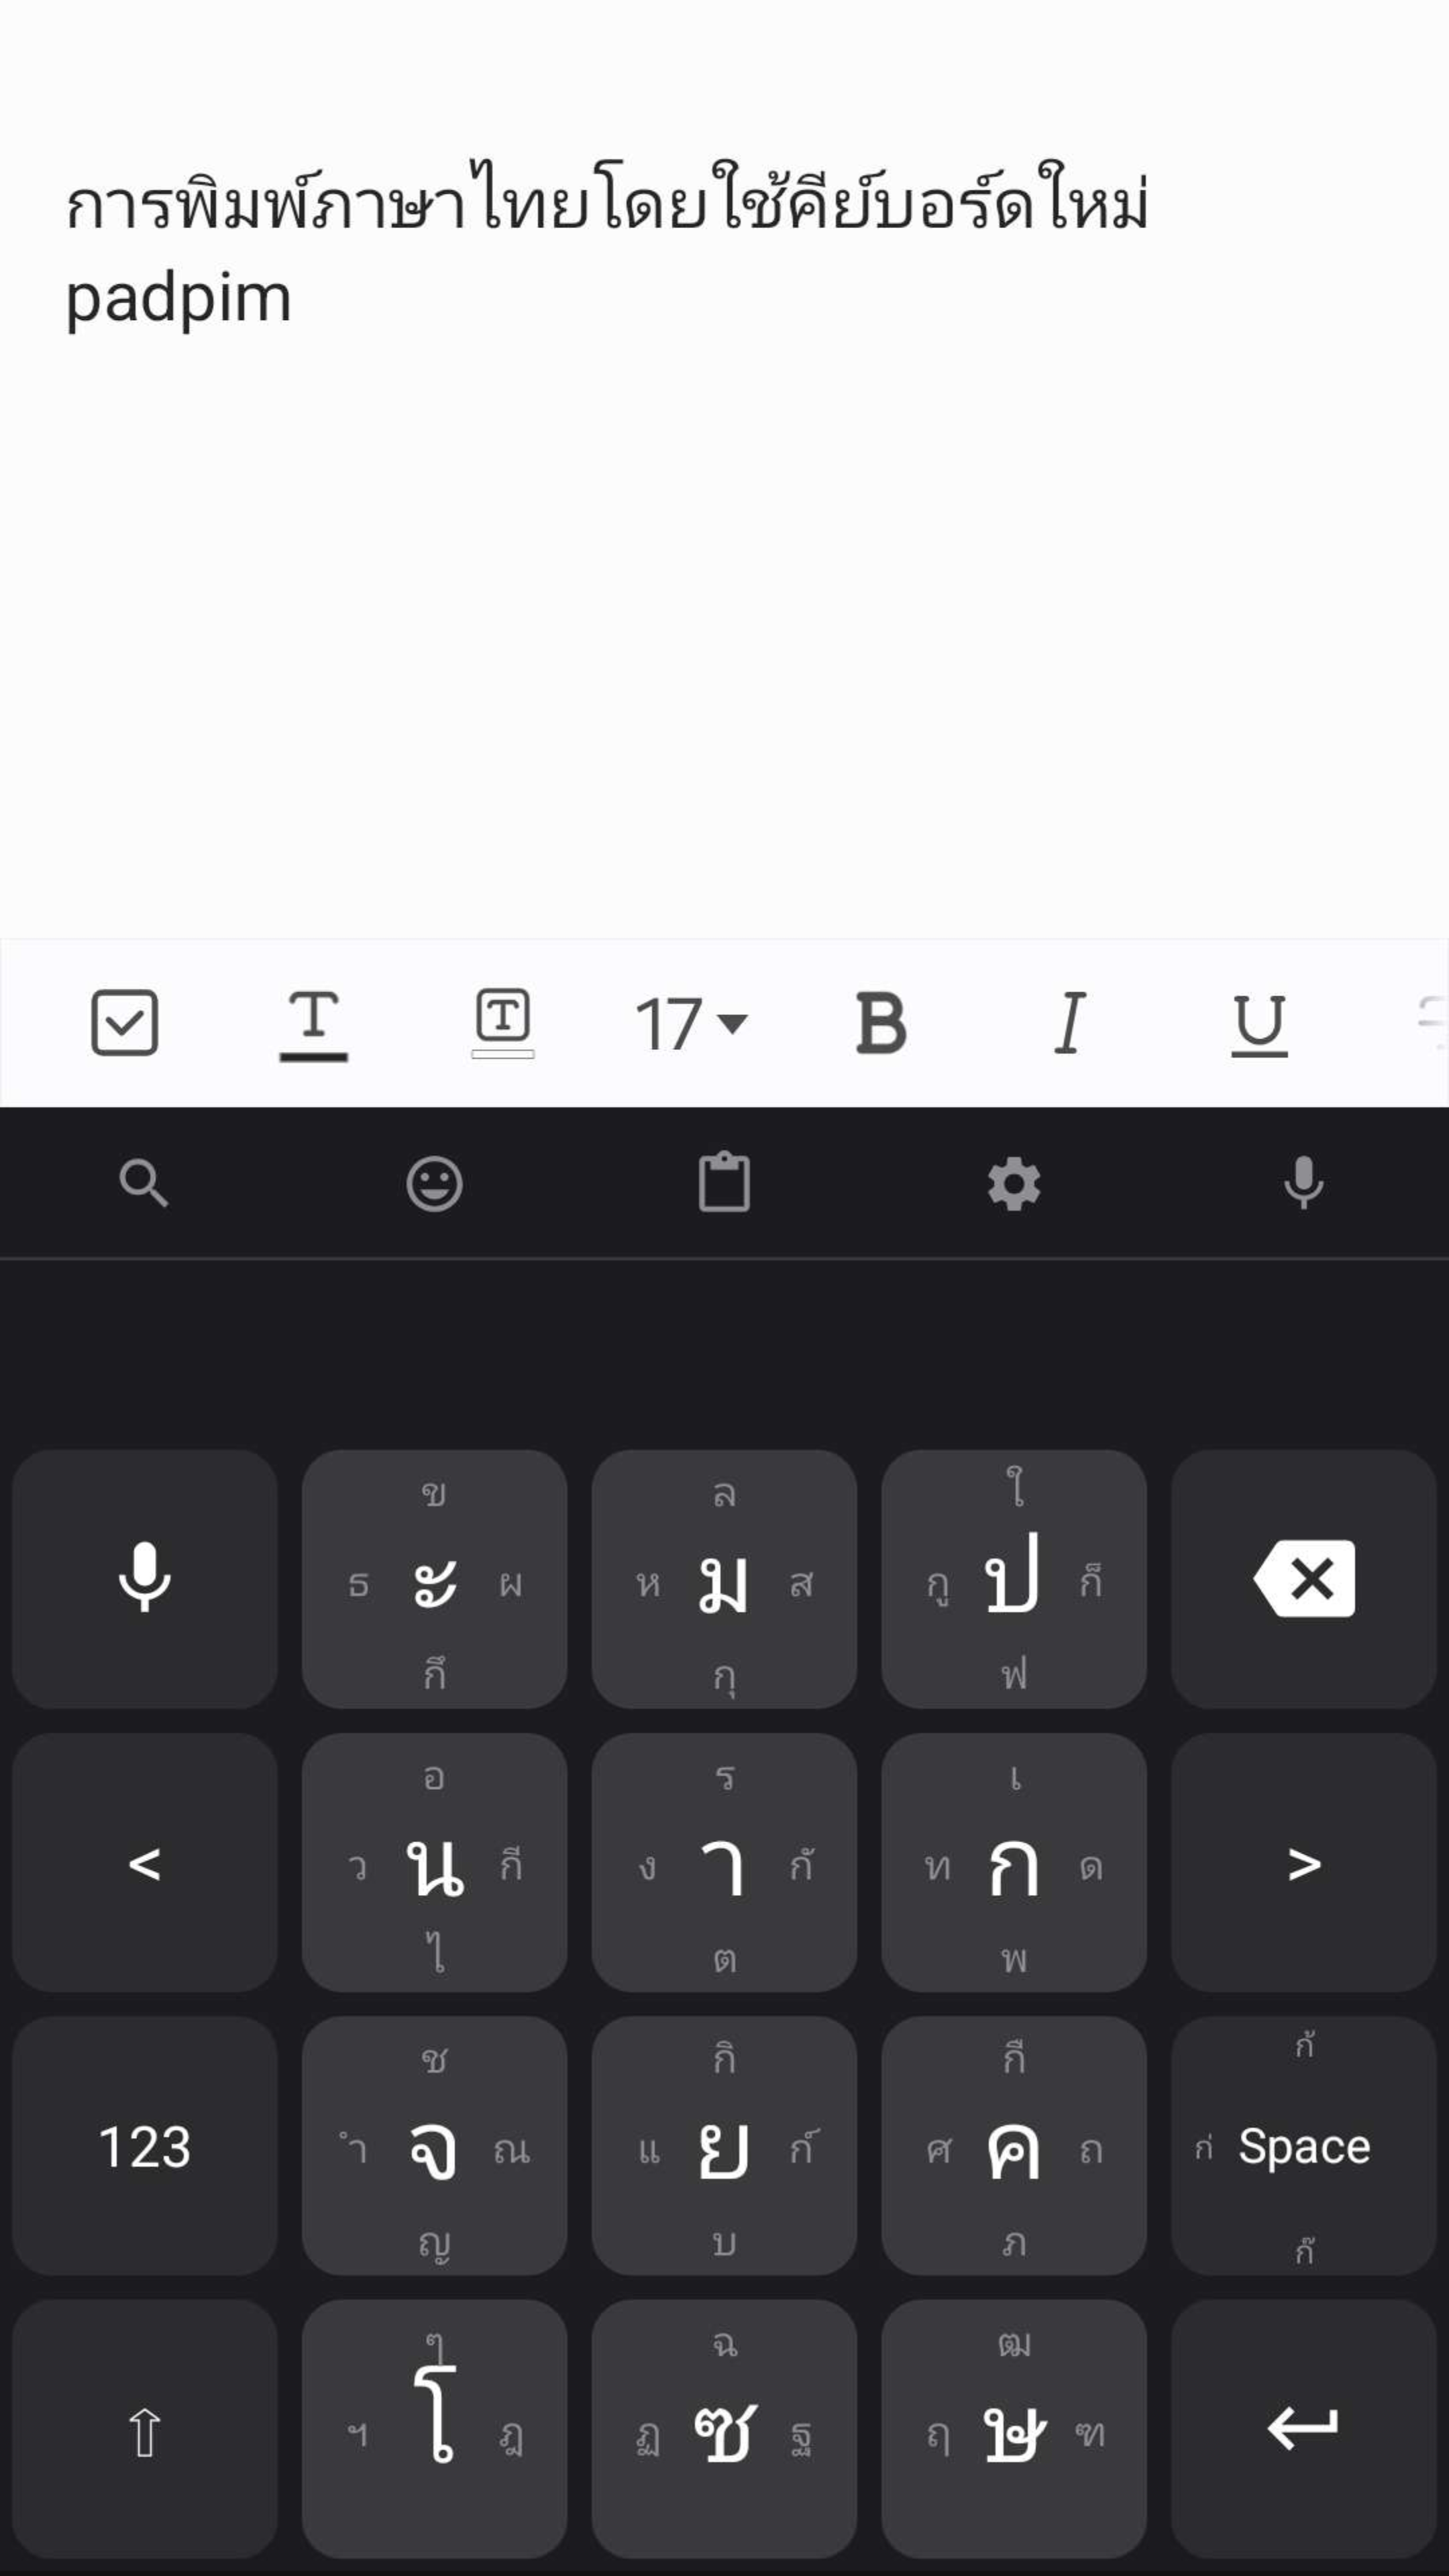
\includegraphics[width=0.75\linewidth]{figures/screenshot.png}
\caption{PadPim Android application showing the PadPim-Opti layout in dark theme. The $3 \times 4$ character grid occupies the center, flanked by utility keys. Each key displays the tap character prominently with flick-direction hints in smaller text at the edges.}
\label{fig:screenshots}
\end{figure}

% ============================================================
\section{Discussion and Future Work}
\label{sec:future}
% ============================================================

\textbf{User study.}
The most critical next step is a formal within-subjects user study comparing PadPim-Opti, PadPim-Key, and Kedmanee QWERTY on:
(1)~typing speed (WPM),
(2)~character error rate (CER),
(3)~subjective preference (NASA-TLX workload assessment), and
(4)~learning curve over a 2--4~week longitudinal period.
We plan to recruit 30+~participants with varying Thai keyboard experience to measure both novice onboarding and expert performance.

\textbf{Bigram-aware optimization.}
The current greedy algorithm optimizes for single-character frequency.
A natural extension is to incorporate bigram transition costs---penalizing the placement of frequently co-occurring characters on the same key or on distant keys.
Metaheuristic approaches (simulated annealing, genetic algorithms) could search the larger combinatorial space that arises when bigram effects are considered~\cite{zhai2002,dunlop2012}.

\textbf{Diagonal flick directions.}
The current design uses 4~flick directions (up, down, left, right).
Adding diagonal directions (up-left, up-right, down-left, down-right) would expand each key to 9~input slots, potentially accommodating more characters on the main page.
However, diagonal flicks may reduce accuracy; this trade-off merits empirical investigation.

\textbf{Personalized layouts.}
Individual users may exhibit different character frequency distributions depending on their communication style, profession, or dialect.
PadPim already supports a custom layout editor; a future version could automatically generate a personalized optimal layout from a user's own typing history.

\textbf{Cross-platform deployment.}
PadPim is currently Android-only.
Porting to iOS (via a custom keyboard extension) and web-based virtual keyboards would broaden the potential user base.

\textbf{Accessibility.}
The large touch targets of a 12-key layout may benefit users with motor impairments.
We plan to investigate PadPim's usability for accessibility use cases in collaboration with occupational therapists.

% ============================================================
\section{Conclusion}
\label{sec:conclusion}
% ============================================================

We have presented PadPim, to our knowledge the first data-driven 12-key flick keyboard designed for Thai script.
By collecting character frequencies from over one million lines of modern Thai conversation, defining a position-scoring model that accounts for both grid ergonomics and flick-direction difficulty, and applying a greedy assignment algorithm, PadPim maps 57~Thai characters onto 12~keys.
Together with three tone marks on the space key, approximately 97.5\% of Thai character occurrences are reachable without a shift layer.

Our results suggest that the Japanese flick-input paradigm transfers effectively to Thai despite the script's 69-character inventory.
The two layout variants---PadPim-Opti for maximum speed and PadPim-Key for easier learning---offer users a meaningful choice.
Compared to the standard Kedmanee QWERTY layout on mobile, PadPim offers 4.2$\times$ larger touch targets, near-unity keys-per-character, and true one-handed operability.

The primary limitation of this work is the absence of a formal user study; the evaluation relies on theoretical metrics.
The open-source Android implementation is available for public beta testing, and we plan a within-subjects user study to empirically validate the efficiency gains reported here.

% ============================================================
% ACKNOWLEDGMENTS
% ============================================================
\section*{Acknowledgments}

We thank the 138 university student volunteers who contributed aggregated character-frequency counts for this research.

% ============================================================
% DATA AVAILABILITY
% ============================================================
\section*{Data and Code Availability}

The PadPim Android application source code is publicly available at \url{https://github.com/Jnx03/ThaiFlickKeyboard}.
The character frequency data used for layout optimization and the layout specifications are documented in the repository under \texttt{docs/layout.md}.
Raw conversation text was not retained; only anonymized, aggregated character counts were collected and used.

% ============================================================
\balance
\bibliographystyle{plain}
\bibliography{references}

\end{document}
